\chapter{結論}
\label{conclusion}

本章では,本研究のまとめと今後の課題を示す.

\section{実験の結果}

この章では本研究の結果について述べる.


\subsection{Case1 }

\section{本研究の課題}

本研究では, 自動車に限りモビリティーの利用者の満足度を高める経路制御を行う機械的な手法に取り組んだ.
しかし,

\subsection{想定環境の複雑化}

本研究では, 事前に選び出した幹線道路とその周辺にある主たる施設のみの仮想環境をソフトウェアで再現した. 
しかし, MaaS社会の実現においては交通機関は自動車以外の鉄道やバスなどの大量輸送型の交通機関との連携も必要だとされている.
今後は鉄道ダイヤやバスとの接続など, 多種の交通機関との連携を考える必要がある.~\cite{MaaSIntegration}

\subsection{モデルアルゴリズムの改良}

本研究では最も基本的なDQNを用いて実験を行った. しかし, DQNをベースとしたアルゴリズムの改良を施すことにより, さらに精度が向上する可能性がある.
現在, DQNをベースとした改良アルゴリズムには以下のようなものがある.


\begin{itemize}
    \item Double DQN
    \item Prioritized Replay
    \item Dueling DQN
\end{itemize}

\subsection{学習器の連携}

本研究では深層強化学習が利用者の満足度を高めるという視点で制御を行えるか実験を行った.
ただ, 実際に本研究の手法を適用する場合, 自動車単体で行動は現実的に不可能である.
従って, DQNによる強化学習器であるエージェントを複数設置する必要がある. 下に示す図~\ref{integrated_dqn}ように環境εを複数のエージェントα, β, Σ, Δ
で共有するマルチエージェントモデルにおいて全体最適が取れるかを検証する必要がある.
なお, 環境εはそれぞれのエージェントから行動aを受け取り, 報酬rを返す点に置いては本研究で用いたものと変わらない.



\begin{figure}[H]
    \centering
    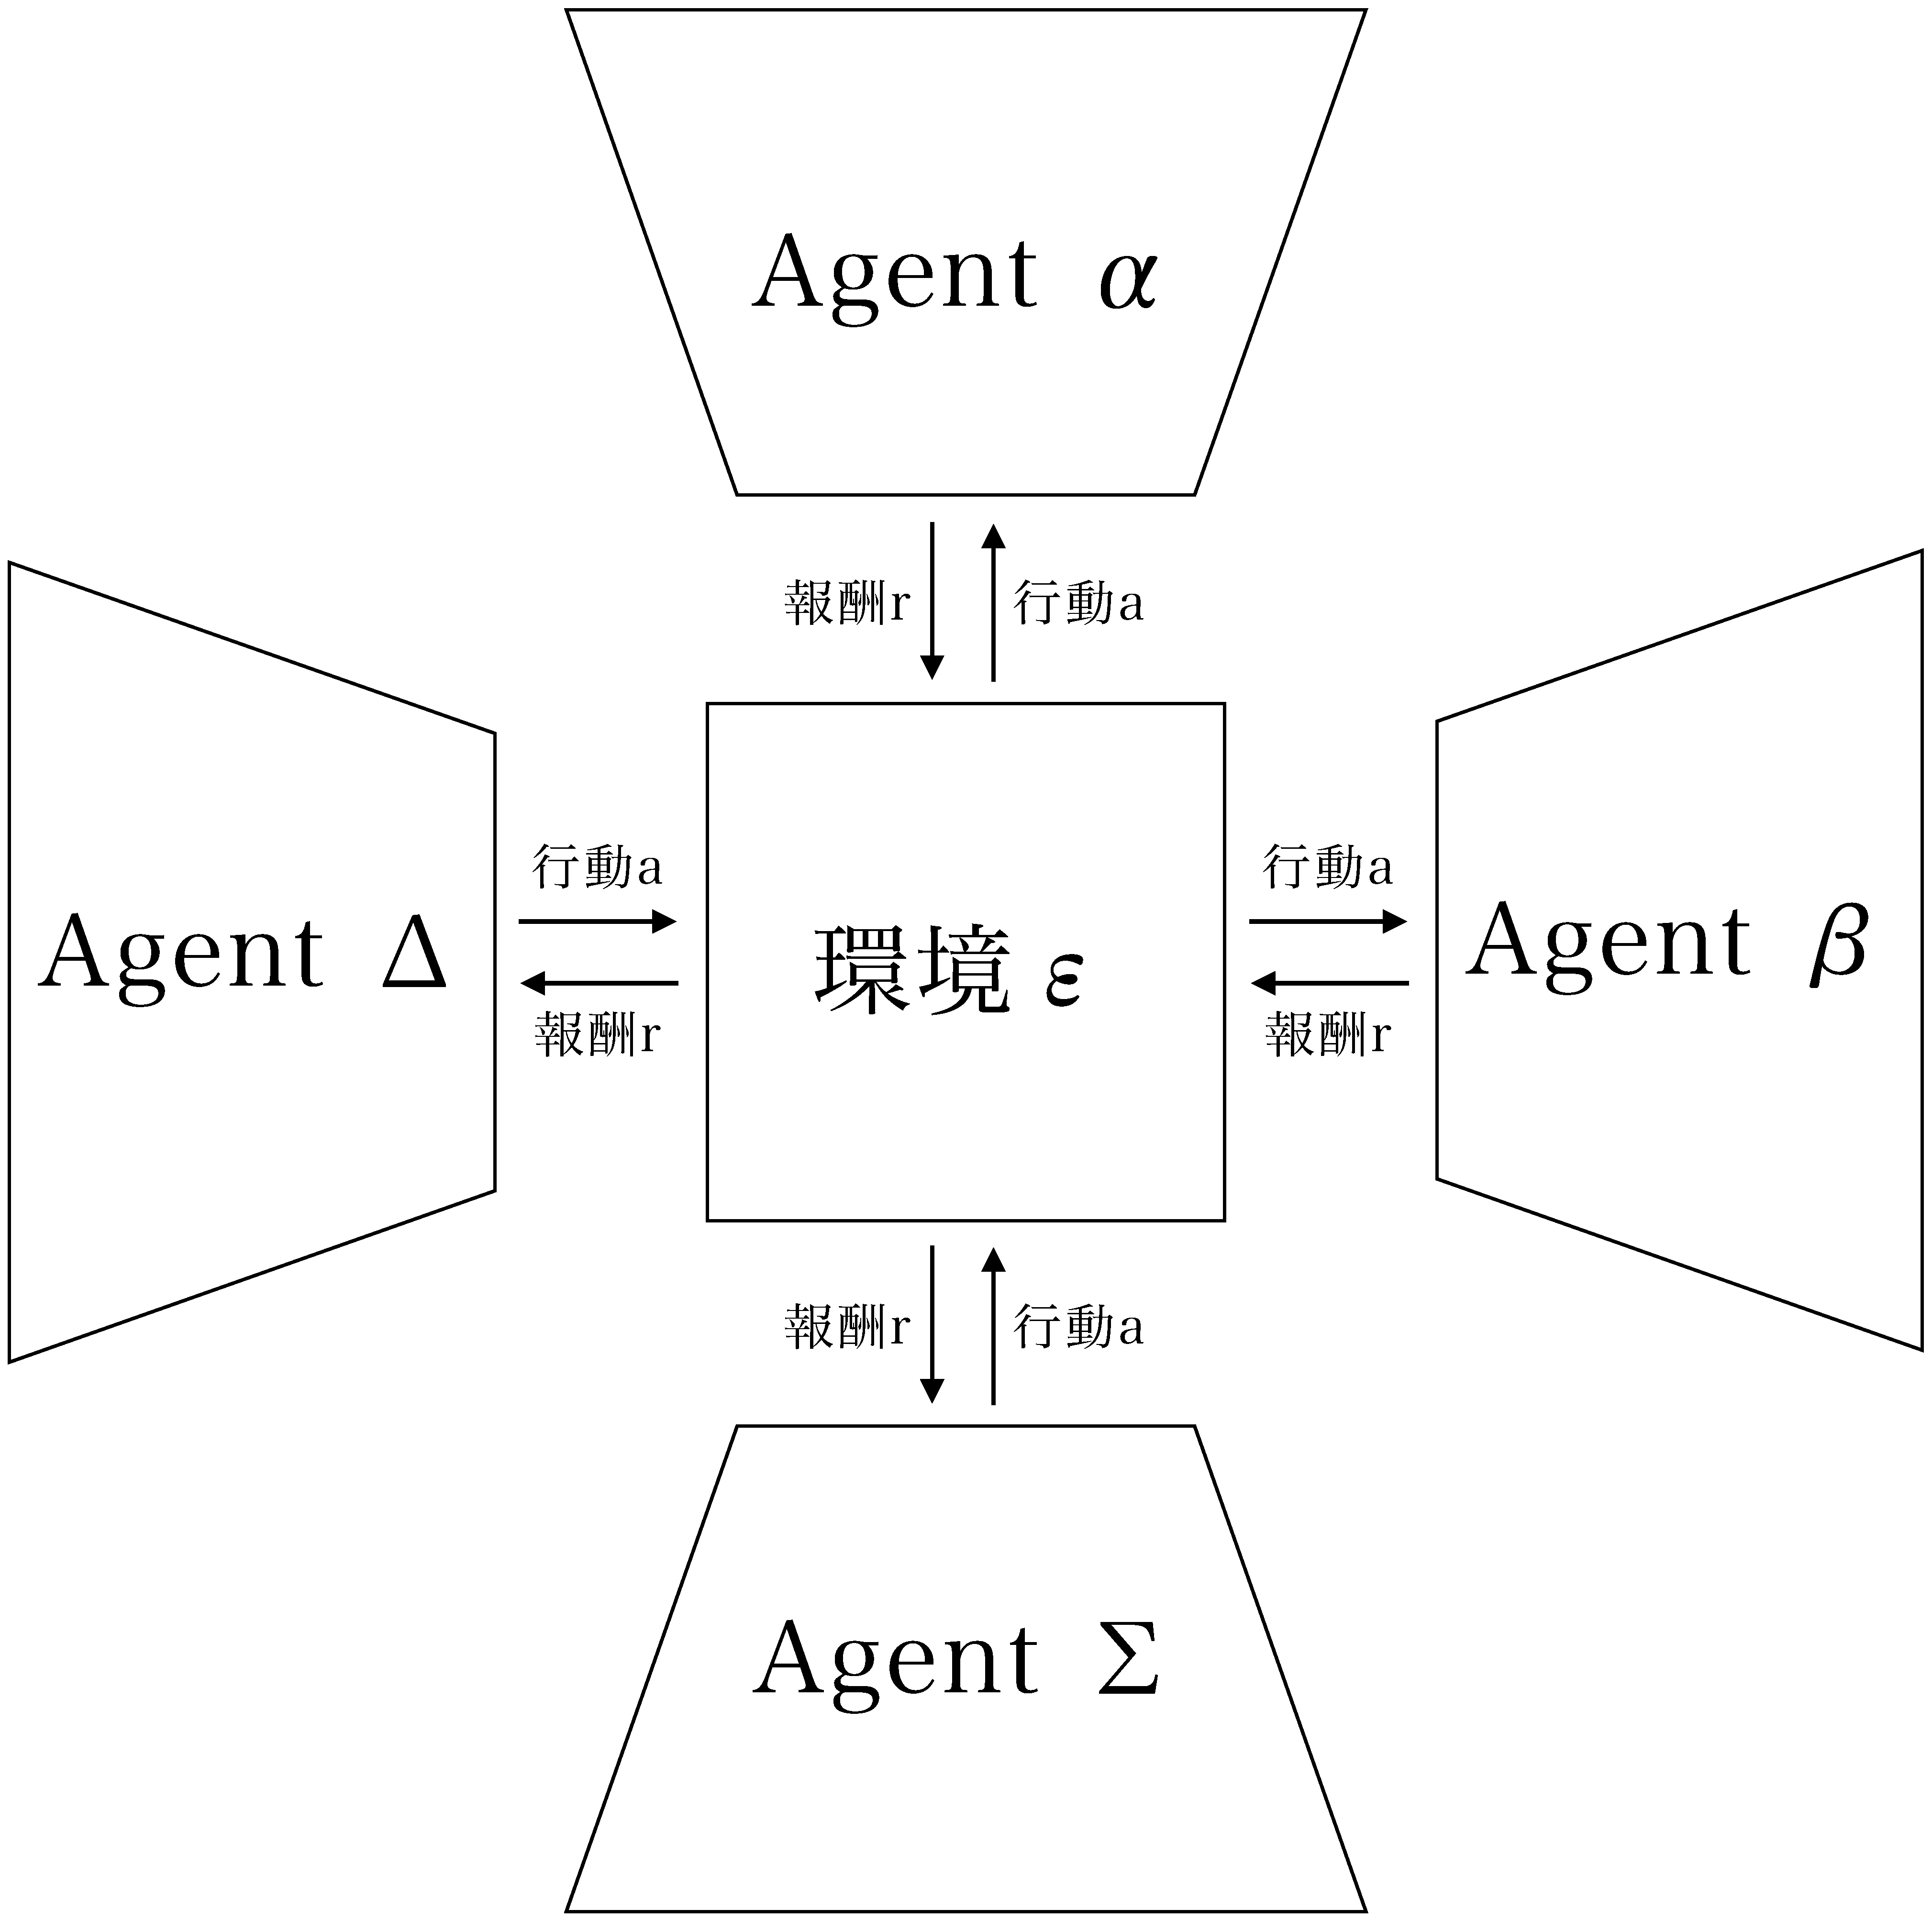
\includegraphics[clip,width = 12.0cm]{assets/multiagent_shared_env.eps}
    \caption{複数エージェントで環境を共有する概念図}  \label{integrated_dqn}
\end{figure}

%%% Local Variables:
%%% mode: japanese-latex
%%% TeX-master: "../thesis"
%%% End:
